
\chapter[Rendering Bread Crumb Geometry]{Rendering Bread Crumb Geometry and Other Porous Materials}
\section{Introduction}

%Los resultados obtenidos son realistas y se renderizan en tiempo real. La misma evita el uso de estructuras intermedias, simplificando el desarrollo y reduciendo los costos computacionales.


The overwhelming variety of materials and their complex light interactions has been a central research topic in Computer Graphics for decades. 
Physics-based modeling may achieve outstanding light transport phenomena, whose computational approximations are a mainstream topic in the current research on rendering.
In complex materials, geometric modeling undergoes a similar research strategy, starting from a Physics-based understanding of the material that further leads to an adequate computational approximation.
Realistic material rendering should take into consideration geometrical modeling and light interaction simultaneously.

The choice of a geometrical model depends on the material and the intended scale representation.
This choice highly influences the rendering algorithm. Main approaches to material rendering include surface or volume treatment. 
The rendering equation \cite{Kajiya1986} models geometrical optics behavior in surfaces. 
The volume rendering equation \cite{Kajiya1984} represents scattering phenomena in volume densities.

Typically, authors use the surface representation for homogeneous materials (metals, plastics, and similar materials) \cite{Neumann1999}.
This method models microscopic surface details using statistical assumptions.
If mesoscopic details are modeled (as required for instance in wood or bricks) \cite{Lefebvre2000}, a usual technique is to precompute these details in textures that can be mapped onto surfaces.
Locally flat surfaces are fast to render but they impose limitations to the rendering quality that are sometimes impossible to surmount, specially the features that arise due to the mesoscopic structure and light transport phenomena in the materials.

Bread crumbs are extremely complex materials to model and render, due to the intricate geometries and light transport phenomena arising within them.
In this particular case, the naive surface approach flatly fails, since mesoscopic details, clearly visible on their surfaces, are essential to recognize the material.
More sophisticated surface modeling techniques, like the use of bidirectional texture functions \cite{Tong2002}, does not handle light propagation phenomena adequately.
To overcome this limitation, a complex material model is proposed \cite{Tong2005}.
This method produces more realistic results, but the capturing and rendering procedure are extremely complex, and the modeling is somewhat inflexible (for example, the surface representation does not allow arbitrary cuts).


On the other hand, there is a wide literature about modeling materials that are better fitted to a volume representation (for example smoke and clouds) \cite{Chentanez2011,Zhou2008}.
Volumes are computationally expensive but, being mesh-free, they do not have the rendering drawbacks mentioned above for surfaces.
There is a trade-off, then, between geometrical representations for complex materials.
Where simplicity and real-time rendering are required, surface-based representation is mostly used, and when photorealism is the final requirement, a volume-based modeling is chosen.
However, the arise of GPUs is shifting this trade-off, since it may allow volume representations at interactive time rates, as we show in this chapter.

In this chapter we apply a GPU based direct volume rendering (DVR) \cite{Levoy1988,Kruger2003, Kratz2006} on a scalar field to render the final structure.
DVR applies a ray marching algorithm through a volume, accumulating different properties for each pixel.
We enhance the rendering method with self-occlusion, specular highlights, automatic crust determination, and shadows.
The rendering workflow does not use intermediate structures, simplifying the modeling process.
In addition, the bread crumb shape can be modified interactively, with the possibility of performing arbitrary cuts and slices of the 3D structure in real time.
Also, the bread crust can be easily defined along with its own properties like color and translucency.


The method obtains very promising images in real time.

\section{Previous Work}
The topic of photorealistic material modeling and rendering attracted a significant amount of research recently.
Most has been focused in frequently appearing complex materials such as water \cite{Schechter2012}, skin \cite{Donner2006}, metals, plastics \cite{Kurt2010}, etc.
The computer graphics community has struggled to adequately emulate the appearance of other materials, such as baked materials ({\em e.g.}, pizza, cookies), but, due to their complex geometry and underlying light transport phenomena, this continues to be an open problem \cite{Voglsam2013}.
Until recently, the computational cost of rendering physically based models of these materials was impractical when real-time is an issue.
However, the remarkable growth in computing power do to the massively parallel design of modern graphics cards \cite{Yeo09,Harris06}, is enabling the simulation of complex light transport phenomena at acceptable computational rates.

Simulating an acceptable bread geometrical model represents an additional challenge.
This and other kinds of porous structures are the result of complex mechanisms involving physical deformations, heat and mass transport during baking, and several chemical reactions.

Recent studies employs phenomenological considerations on real breads, but the geometry is fixed ({\em i.e.}, non procedural) \cite{VanDyck2014}: a fixed geometry does not allow to obtain several different bread types easily, since it requires a capture procedure for each of them, and, in addition, bubble distributions can be neither controlled nor changed.

The presence of mesostructures (bubbles and alveoli of complex shapes) makes bread a quasi homogeneous material \cite{Tong2005}. 
For this reason, adequate surface representations of this material are not possible.
Typical techniques such as Bidirectional Reflectance Distribution Functions (BRDFs)
\cite{Kurt2009}, and Bidirectional Surface Scattering Reflectance Distribution Functions (BSSRDFs) \cite{Donner2009}, are not satisfactory.
A material model \cite{Tong2005} solves these limitations, but the associated drawbacks (complex capture procedure involved, computational costs, poor geometry variability),
makes the method far from practical.

On the other hand, research on physically inspired mathematical models of bread crumbs is not uncommon in the food industry related literature.
These works aim to adequately model and simulate heat and mass transfer in dough during baking, among other issues.
Recent results suggest that 1D models could suffice, for instance modeling the geometry as an infinite cylinder, or assuming only one radial coordinate \cite{Purlis2012, Thorvaldsson1999}.
These and other results in the food industry have some significance in bread crumb modeling and rendering, and may be used as a further basis for computational baking models. 


\section{Direct Volume Rendering (DVR)}
The technique of DVR\cite{Kratz2006} generates two-dimensional images by computing the interaction of light with a semi-transparent medium that is represented by a discrete scalar field.
This field describes the density of the medium at regular sample points. 
For each pixel in the image a ray is cast from the camera position and the radiance reaching the camera from its direction is computed by approximating the radiative transfer equation (RTE). This equation describes the change in radiance along a ray as it traverses non-transparent media.
In its complete form, the RTE incorporates many different optical properties and effects. 
In order to approximate the result of the RTE in real-time, this work uses a simplified version of the equation that only incorporates some of the optical phenomena that occur in reality.

There are three important optical phenomena that affect the propagation of light through a medium at a given point in space: emission, absorption and scattering.
Emission is the generation of radiant energy in a given direction.
Absorption happens when a fraction or all of the radiant energy in the light ray hits an opaque object and is transformed into other forms of energy. 
%
Finally, scattering events result in the change of direction of photons. 
Scattering events that cause photons to change directions away from the direction of a ray are called out-scattering events. Conversely, in-scattering events result in photons changing direction towards the ray direction.
%
The contribution of in-scattering is often computed for radiance from a single direction which corresponds to the main light source of the scene.
This corresponds to the radiative energy arriving at a point from the light source, bouncing on the particles in the medium at that point and then traveling along a given ray direction.

The RTE can be summarized as:

\begin{equation} \label{eq:general_radiance}  
  L(p_n) = L_b + \int_{p_0}^{p_n} \frac{\partial L(t)}{\partial p} \, dt,
\end{equation}

\noindent where $L_b$ is the background radiance, and $p_0$, $p_n$ are the closest and furthest visible points along the ray direction, respectively, $L(t)$ is the radiance at point $t$, and $\partial p$ is the distance between sampled points. 
Since the input to the DVR algorithm is a discrete data set, in order to compute $L(p_n)$ the integral is approximated by a sum.

Extinction is the decrease in radiance in a ray due to absorption and out-scattering.
We can approximate this effect by defining an absorption coefficient for the media, $k_a$ and an out-scattering coefficient $k_s$. 
If we neglect the out-scattering effect, the formula that describes the radiance reaching a point after traversing a ray segment is:

\begin{equation} \label{eq:radiance_absorption}  
    L_b \ e^{- \textstyle  \int_{p_0}^{p_n} k_a(t) \, dt}.
\end{equation}

We introduce the value $\int_{p_i}^{p_j} k_a(t) \, dt$, the absorption coefficient, and we will refer to it as $\tau_{(p_i, p_j)}$. 
Transmittance is complementary to extinction. It describes the amount of light passing through a medium in a given direction. 
The transmittance value along two points $p_i$ and $p_j$ is thus:

\begin{equation} \label{eq:transmittance}  
  T(p_i,p_j) = e^{- \textstyle \tau_{(p_i, p_j)}}.
\end{equation}

If we assume that at every point inside the volume along the ray there is an increase of radiance due to emission and in-scattering phenomena ($\rho$), then our initial radiance estimate becomes:

\begin{equation} \label{eq:ray_radiance}  
  L(p_n) = L_b \ e^{-\tau(p_0, p_n)} + \int_{p_0}^{p_n} \rho \ e^{-\tau(t,p_n)} \, dt.
\end{equation}


This means that the radiance along points $p_0$ and $p_n$ is the attenuated remaining background radiance plus the attenuated emission and in-scattering at every ray point.
The DVR algorithm samples the volume density function at regular intervals, approximates the transmittance along those points and computes the amount of light reaching the camera along the ray direction.
The computation replaces the integral sum by a discrete sum over the length of the ray intersecting the volume:

\begin{equation} \label{eq:ray_radiance}  
  L(p_n) = L_b \ e^{-\tau(p_0, p_n)} + \sum_{p_0}^{p_n} \rho \ e^{-\tau(p_i,p_n)}.
\end{equation}

Other effects can be accounted for, augmenting the final image's fidelity, as well as the technique's computing cost. 
The basis of our rendering algorithm uses the simplified transmittance and emission only model, along with some artistic considerations, to achieve real time frame rates.
The rendering algorithm is described in detail in a further section. 

\section{Implementation}


We created a demo application \footnote{available at \emph{https://www.github.com/rbaravalle/Pysys}} that uses the particle system described in the previous sections to render real-time bread models using a DVR approach. 
In this demo we produced a volume texture from the original particle system.
A cube that corresponds to this volume is then rendered in the scene.
The material used to render the cube uses a very simple vertex shader and a fragment shader that implements the DVR algorithm. For each fragment, this shader computes a ray originating from the camera position and in the direction of the fragment that must be shaded. 
The procedure samples the volume texture at regular intervals along the intersection of this ray and the cube.
The sample values are then used as input of a simplified version of the radiative transfer equation to compute the resulting pixel color as described in previous sections.
%~\ref{sec:DVR}.
We employ these equations to accumulate the transmittance of the ray and the radiance contribution at every sample point.
The computation ends if the transmittance falls below a threshold value or if the ray exits the cube. 
Single in-scattering is approximated by computing a secondary ray at each sample point directed towards the scene light source.
This secondary ray is then sampled to determine the amount of light that reaches the original sample point. 
This technique allows to naturally perform self shadowing within the model.

We shade the pixel using the primary and secondary ray transmittance information. 
At this point, different artistic considerations may be applied to yield different
looking materials.
For instance, we can differentiate crumb and crust by assigning a higher extinction coefficient and a darker color to crust regions. 
A soft yellowish color applied in other regions provides a crumb appearance.
Additionally, it is possible to add a faint specular reflection. 
The contribution of that reflection is computed at the first intersection point between the ray and the particle system in order to increase the final image realism. 
The normal vector used for this computation is the gradient of the volume texture at that point.

The demo we present provides the user with the ability to modify parameters such as the transmittance coefficient, the transmittance threshold, the color assigned to the crumb and the visibility of the specular highlights. 
By modifying these parameters the user can produce images that resemble other porous materials, such as sponges.

\subsection{Ambient Occlusion}

One key aspect to enhance the final image appearance is the local contributions due to tiny material features (emission, occlusion, absorption). 
Previous works show that considering ambient occlusion can greatly enhance synthetic image realism \cite{Hernell2010}.
Based on this idea we approximate multiple in-scattering by computing (offline) an ambient occlusion term for each voxel in the scalar field and storing it as an additional volume texture, which is used by the fragment shader.

For each voxel, the algorithm sets a neighborhood of radius $r$ and stores the mean voxel value within that radius in the ambient occlusion texture.
It then uses this value to modulate the contribution of a ray sample.
Setting different values for $r$ produces similar results. 
Fig.~\ref{fg:occlusion} shows that the enhancement added using ambient occlusion clearly improves the final image appearance and is a key aspect in realistic bread appearance. It is worth mentioning that the net effect of this term was somehow oblivious to the radius $r$ of the surrounding sphere, for $r > 0$.
 
\subsection{Normals Computation}

We use a simple forward difference schema for the gradient computation. In this method, we compute the normal vector at a point using the gradient, represented as the normalized difference vector between the field values at the forward positions and the actual position:

\begin{equation}
\begin{aligned}
x &= tex(pos+(1,0,0)) - tex(pos)\\
y &= tex(pos+(0,1,0)) - tex(pos)\\
z &= tex(pos+(0,0,1)) - tex(pos) \\
N &= normalize([x,y,z])
\end{aligned}
\end{equation}

We use the normals and the light vector to determine the specular contribution, applying a simple Phong model \cite{Phong1973}, with a parameter that lets the user change the impact of the specular component.
We tested other more accurate specular models, but there was no appreciable difference in the final bread appearance.

\subsection{Shadows Computation}

The DVR technique can also be used to compute realistic shadows using shadow maps \cite{Williams1978}.
During the shadow map generation we again render a cube representing the particle system.
The fragment shader for that box uses the same ray-casting method explained above, but only computes the transmittance along the ray. 
If the transmittance along the ray is above a threshold value, then the fragment does not correspond to an occluder and its depth is set at infinity. 
If during the volume traversal the transmittance falls below the threshold, the fragment depth is set to that sample point depth.
This technique is used along with percentage-closer filtering to generate realistic looking shadows in our demo application.

\subsection{Crust}
We can provide a function that defines whether a volume point is part of the crust or the crumb. For instance, we may provide a function that defines a cylindrical crust envelope by assigning crumb to positions close to the axis of the cylinder, and crust to all other positions. Another function is provided to define whether a point should be considered empty air.
This allows an easy way to define bread crust and slices (see Figs.~\ref{fg:crumb} and \ref{fg:results2}).

\paragraph{Crust determination using Mathematical Morphology}
Since it is difficult or impossible to define mathematical functions that adapt to arbitrary shapes, we propose an automatic method for crust determination using mathematical morphology \cite{Gonzalez2001}.
The idea is to obtain an outer region of the resulting $3D$ scalar field. 
For this, we use basic techniques known as closing, erosion and dilation.

For the purposes of our work, we will define the operations on $3D$ binary scalar fields.
A structuring element $E$ is defined as a binary scalar field representing a particular shape (cube, sphere, etc.).
Structuring elements are employed to perform morphology operations.

The erosion operation can be employed to reduce the total size of a scalar field.
The erosion of a $3D$ scalar field $A$ using a structuring element $B$ is defined as:

\begin{equation}
A \ominus B = \{z\in \mathbb{Z}^3 | B_{z} \subseteq A\},
\end{equation}

\noindent where $B_{z}$ is the translation of $B$ by the $3D$ vector $z$.

The dilation operation is used to augment the total size of a scalar field following its boundary.
The dilation of a $3D$ scalar field $A$ using a structuring element $E$ is defined as:

\begin{equation}
A  \oplus E = \bigcup_{e\in E} A_e.
\end{equation}

The closing operation is used to fill holes in the scalar field.
The closing of a $3D$ scalar field $B$ using a structuring element $E$ is defined as a dilation followed by an erosion:
\begin{equation}
B \bullet E = (B \oplus E) \ominus E,
\end{equation}
see \cite{Gonzalez2001} for further details.

To obtain the outer region of the $3D$ porous volume, we have to eliminate the holes in the scalar field (bubbles) and then compute a boundary.
To do this, the first step performs a closing $c$ of the scalar field using a cube (structuring element of radius $r$), causing the closing of interior bubbles.
Calling $d$ the dilation of $c$ with an spherical element of radius $r_{2}$ and $e$ the erosion $d$ using a spherical structuring element with a slightly shorter radius ($r_{3}$).
The difference between $d$ and $e$ lies in the boundary of the scalar field, so it could be used as a crust.
To eliminate some possible inaccuracies resulting from previous steps, we successively perform a closing of $d-e$ and a dilation to the result, obtaining the final crust.
Fig.~\ref{fg:crusts} shows examples of scalar fields with crusts added using this technique. The results naturally adapt to any scalar field, even with holes.
Since the result would completely cover the scalar field, the crust can be set to span only a subset of the complete volume, allowing the user to see the bread crumb.


\begin{figure}
  \centerline{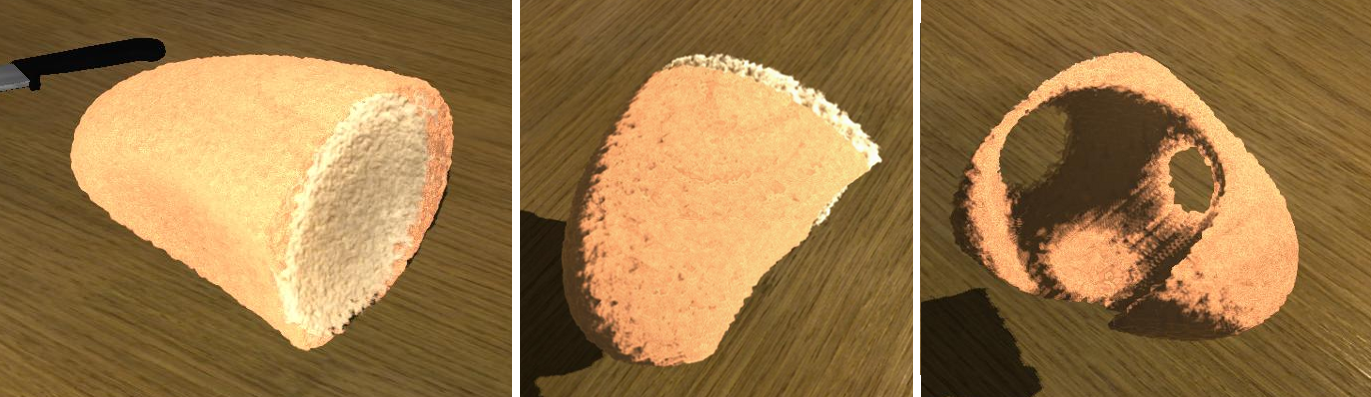
\includegraphics[width=13cm]{figures/crusts}}
  \caption{Crust determination using mathematical morphology. The right image shows that the method works even in extreme cases where the scalar field has holes. }
  \label{fg:crusts}
\end{figure}

\begin{figure*}[htb!]
  \centerline{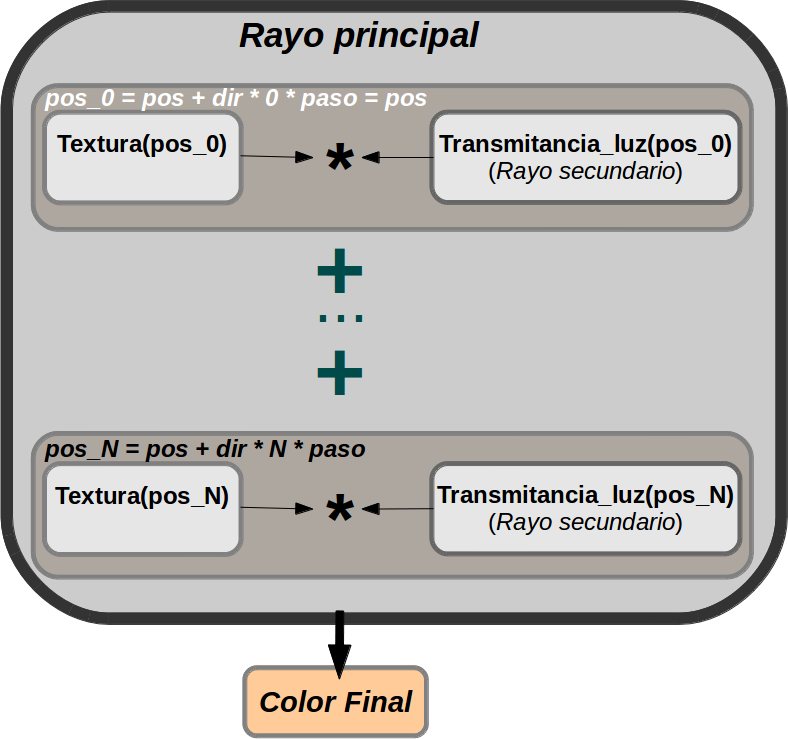
\includegraphics[width=13cm]{fragmentshader}}
  \caption{Cálculo de color en el shader de fragmentos. }
  \label{fg:fragmentshader}
\end{figure*}



\section{Results}


We employed a nVidia GTX 480 ($480$ shader units), which is a typical user configuration.
The CPU is an Intel(R) Core(TM) i5-2300 CPU (quad core).
The screen resolution is $1440\times900$.
In fig.~\ref{fg:application} we show a real-time rendered bread.
Different kinds of bread can be easily modeled changing the parameters of the algorithms (see Fig.~\ref{fg:crumb}).
In Fig.~\ref{fg:results2} we added crust to enhance the final results. 
We also synthesized sponges (see Fig.~\ref{fg:sponges}) with yet different parameter values.
They were easily derived by changing the color and the structure of the volume.
Since yeast is unnecessary in the sponge manufacturing process, we used a random volume texture as a geometry.

We also handled back illumination in the model (see Fig.~\ref{fg:backillum}): the render shows the light propagation in the medium when illuminated from behind.
This is a natural consequence of the RTE based algorithm and the choice of the volume representation that we made.

El programa de prueba creado permite modificar parámetros tales como el coeficiente de transmitancia del pan, el límite de transmitancia, el color asignado a la miga y la intensidad de los reflejos especulares, entre otros.

\begin{figure*}[htb!]
  \centerline{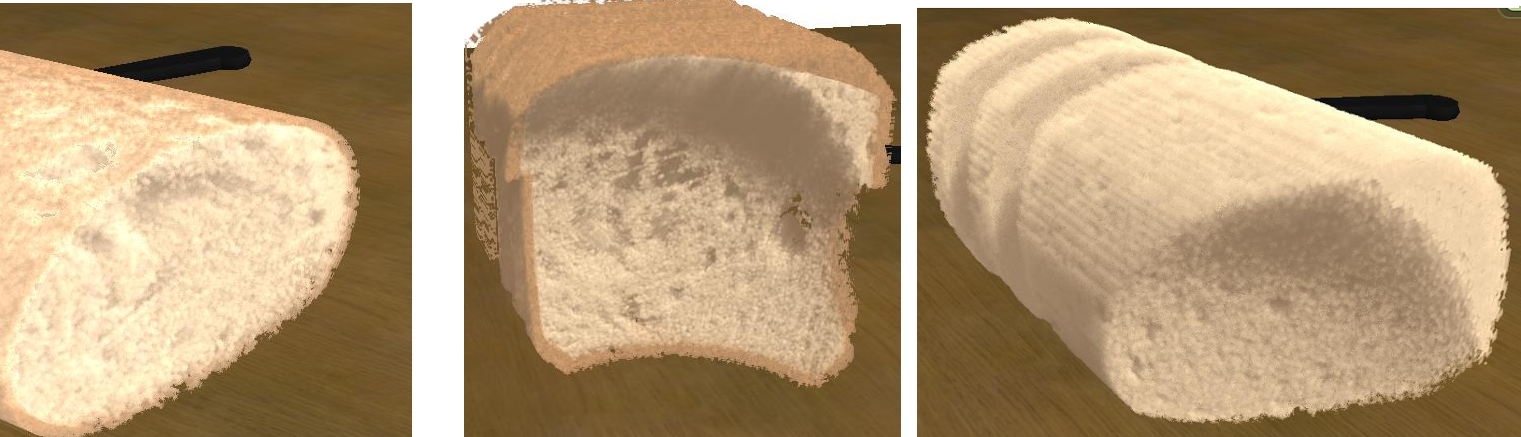
\includegraphics[width=13cm]{fig5}}
  \caption{Different real time rendered breads. The rightmost image shows a bread withouth crust.}
  \label{fg:fig5}
\end{figure*}

\subsection{Other Materials}
It is possible to obtain other porous materials (see Fig.~\ref{fg:fig6}).
These images are the result of a variation in artistical and technical model parameters.
In the leftmost image, a pudding can be distinguished.
The middle image shows a piece of cake.
The right image show a sponge.
It is worth mention that the density function for the sponge is a volumetric texture, which values come from a random function, since the sponge making process is quite different and does not present big alveoli. 
Retro-illumination is approximated in the model, see Fig.\ref{fg:fig7}
The image shows a sponge between the camera and the light source, with beams of light escaping from the sponge and reaching the camera.

\begin{figure*}[htb!]
  \centerline{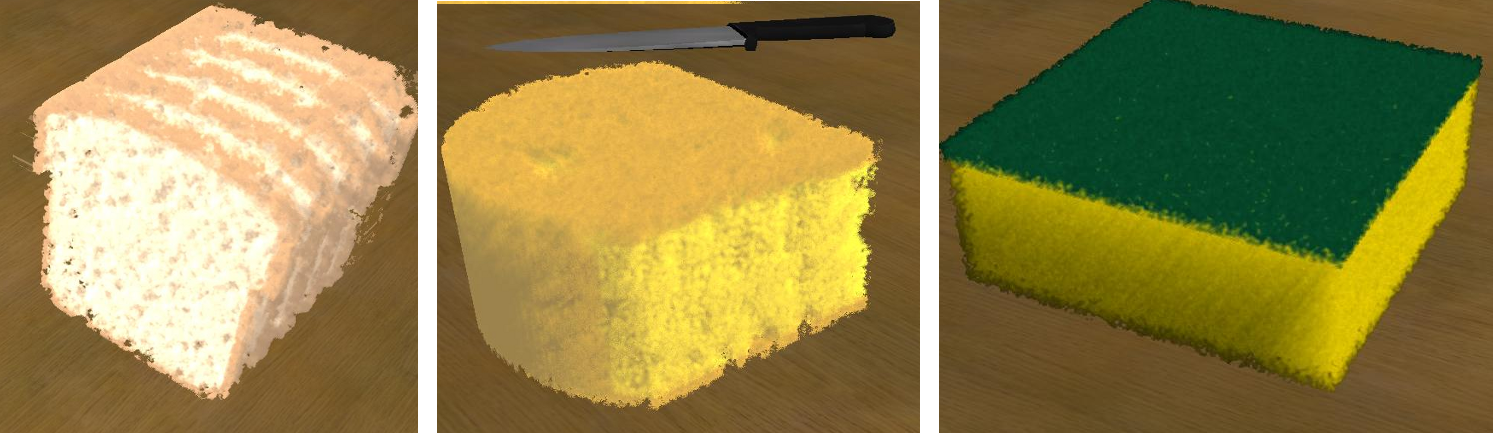
\includegraphics[width=13cm]{fig6}}
  \caption{Different materials obtained with different parameter configurations. From left to right: pudding, cake and sponge.}
  \label{fg:fig6}

\end{figure*}

\begin{figure*}[htb!]
  \centerline{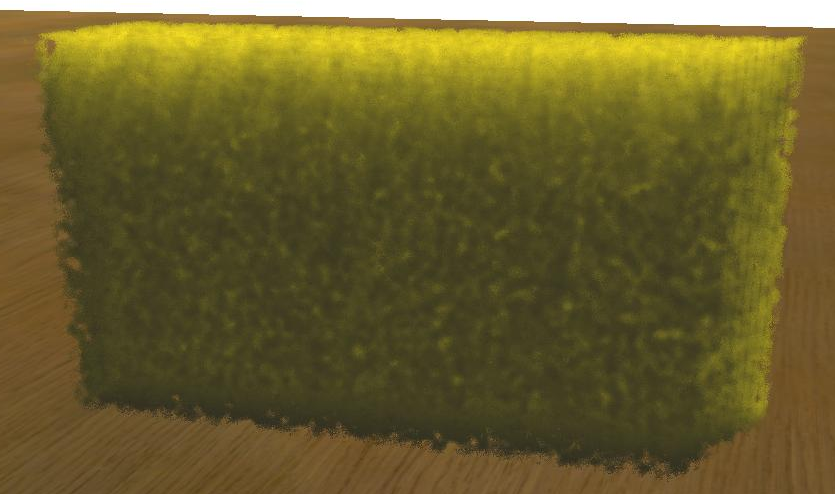
\includegraphics[width=8cm]{fig7}}
  \caption{Retro illuminated sponge.}
  \label{fg:fig7}
\end{figure*}


\section{Computing times}

We rendered all images in real time (FPS over 30). Two parameters are responsible for most of the computations: the transmittance coefficient and the step count.
A low transmittance produces a more transparent material making the ray accumulate more information.

The step count is crucial since for each step we compute the transmittance to the light using a secondary ray.
We experimentally found that values above $140$ give reasonably images for sponges but we needed at least $300$ steps to get a reasonably bread appearance, see Fig.~\ref{fg:stepcount}.
The process automatically scales with the number of GPU processors, so the fps count will increment in more powerful GPUs. 
The use of crust slightly boosts the performance since the transmittance is lower for crust regions, {\em i.e.}, the rays need lower step counts to reach a threshold opacity level.

%\begin{table}[htb]
%\centering
%\begin{tabular}{|c|c|c|c|c|c|c|}
%\hline
% Pasos del rayo         & 128 &  256 \\
%\hline
%\hline
% Tiempo total shaders   & 10 ms &  32.5 ms \\
%\hline
% Rayo Principal         & 2 ms  & 5 ms  \\
%\hline
% Rayos Secundarios      &  8 ms & 27.5 ms  \\
%\hline
%\end{tabular}
%\caption{Detalle de tiempos de renderizado en milisegundos.}
%\label{tab:n2}
%\end{table}




\section{Discussion}

To the best of the authors' knowledge, this is the first attempt to convincingly render bread crumb and other materials in real time without introducing complex intermediate processes (capture, mesh generation, precomputation, post-process).
There are few previous approaches to bread rendering. An example is \cite{Cho2007}, but comparisons with this technique could not be established since key details are unexplained (computing times, render method).
The proposed method is compatible with current rasterization-based real-time GPU rendering pipelines, providing a realistic looking material, and can be easily integrated into  shader-based 3D engines.
Also, the presented shadow mapping technique allows a natural integration of the volume within scenes. 

The modeling and rendering algorithms are flexible enough to model different materials like bread or sponges, changing a few parameters.
Other materials such as cakes, pizzas and cheeses can be implemented in the same way, allowing to manage several materials using the same method.
Also, our volume representation method allows to make real time cuts in the bread crumb.
This is clearly useful in many applications, for instance in video games.

Regarding the illumination model, the success of our algorithms in rendering realistic bread crumbs and other materials could be attributed to the improvements we added to the basic DVR algorithm.
A remarkable improvement in the final realism was due to the addition of an ambient occlusion term, giving the texture a more rich and complex appearance.
Other effects, such as the Phong specular component, enhanced the bread crumb final appearance.
More sophisticated specular methods (for instance, Cook-Torrance model \cite{Cook1982}) did not add a significant improvement.

Computing times were adequate for real-time rendering in standard off-the-shelf computers (we employed a nVidia GTX 480 GPU with an Intel(R) i5 processor).
Reasonable framerates are always achieved except when the rendered object encompasses a big portion of the screen, since the approach is largely fragment-shader bound.
The final framerate also depends on the step count and the transmittance coefficient.
In addition, different materials require different computing costs for rendering.
For instance, an adequate step count to simulate sponge is lower than the bread crumbs step count.
This can be attributed to the fact that the method needs more steps to capture the macroscopic bread bubbles in crumb.
So far, with current off-the-shelf hardware, our method is limited in the final 3D resolution of the material when real-time applications are required.
In other words, drastic close-ups to the structure could lead to homogeneous areas.
This limitation is tied to the GPU texture size, and will be eventually circumvented with next generations of hardware.
In off-line applications, memory swap procedures allow more satisfactory 3D resolutions.


\section{Conclusions}

In this chapter we applied the transmittance direct volume rendering model using the GPU to a 3D scalar field representing the bread crumb structure, obtaining realistic bread crumb images.
We modeled this structure using particle systems and dynamical systems.
We employed a numerical simulation to solve the resulting set of equations which represents the dynamical system. 
The particles avoided each other and grew following the dynamic system.
The modeling algorithm was easily implemented. 
We implemented the render algorithm in the fragment shader using specular and diffuse components, ambient occlusion and automatic crust determination.

Results showed high fidelity images in real time, suitable for application in several areas, such as video games, serious games \cite{Susi2007} and photorealistic rendering. 
These techniques are much simpler and does not present the drawbacks of other state of the art methods, such as capture processes or mesh generation.
These results make us believe that the volume representation is a right choice for bread modeling and rendering.


\begin{figure}
  \centerline{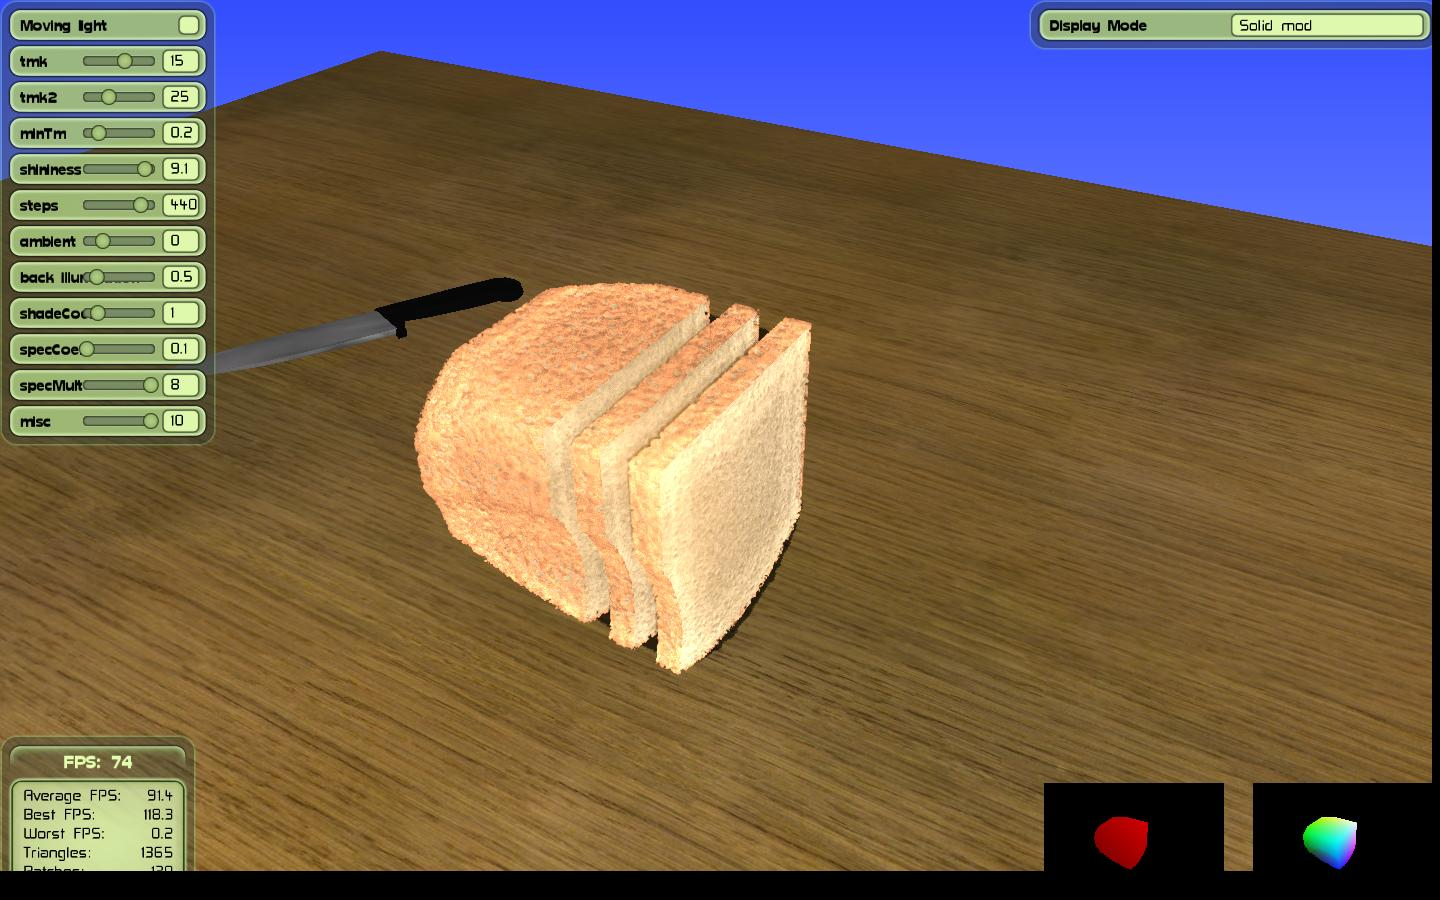
\includegraphics[width=13cm]{figures/application}}
  \caption{Our demo application showing a real time rendered bread.}
  \label{fg:application}
\end{figure}

\begin{figure}
  \centerline{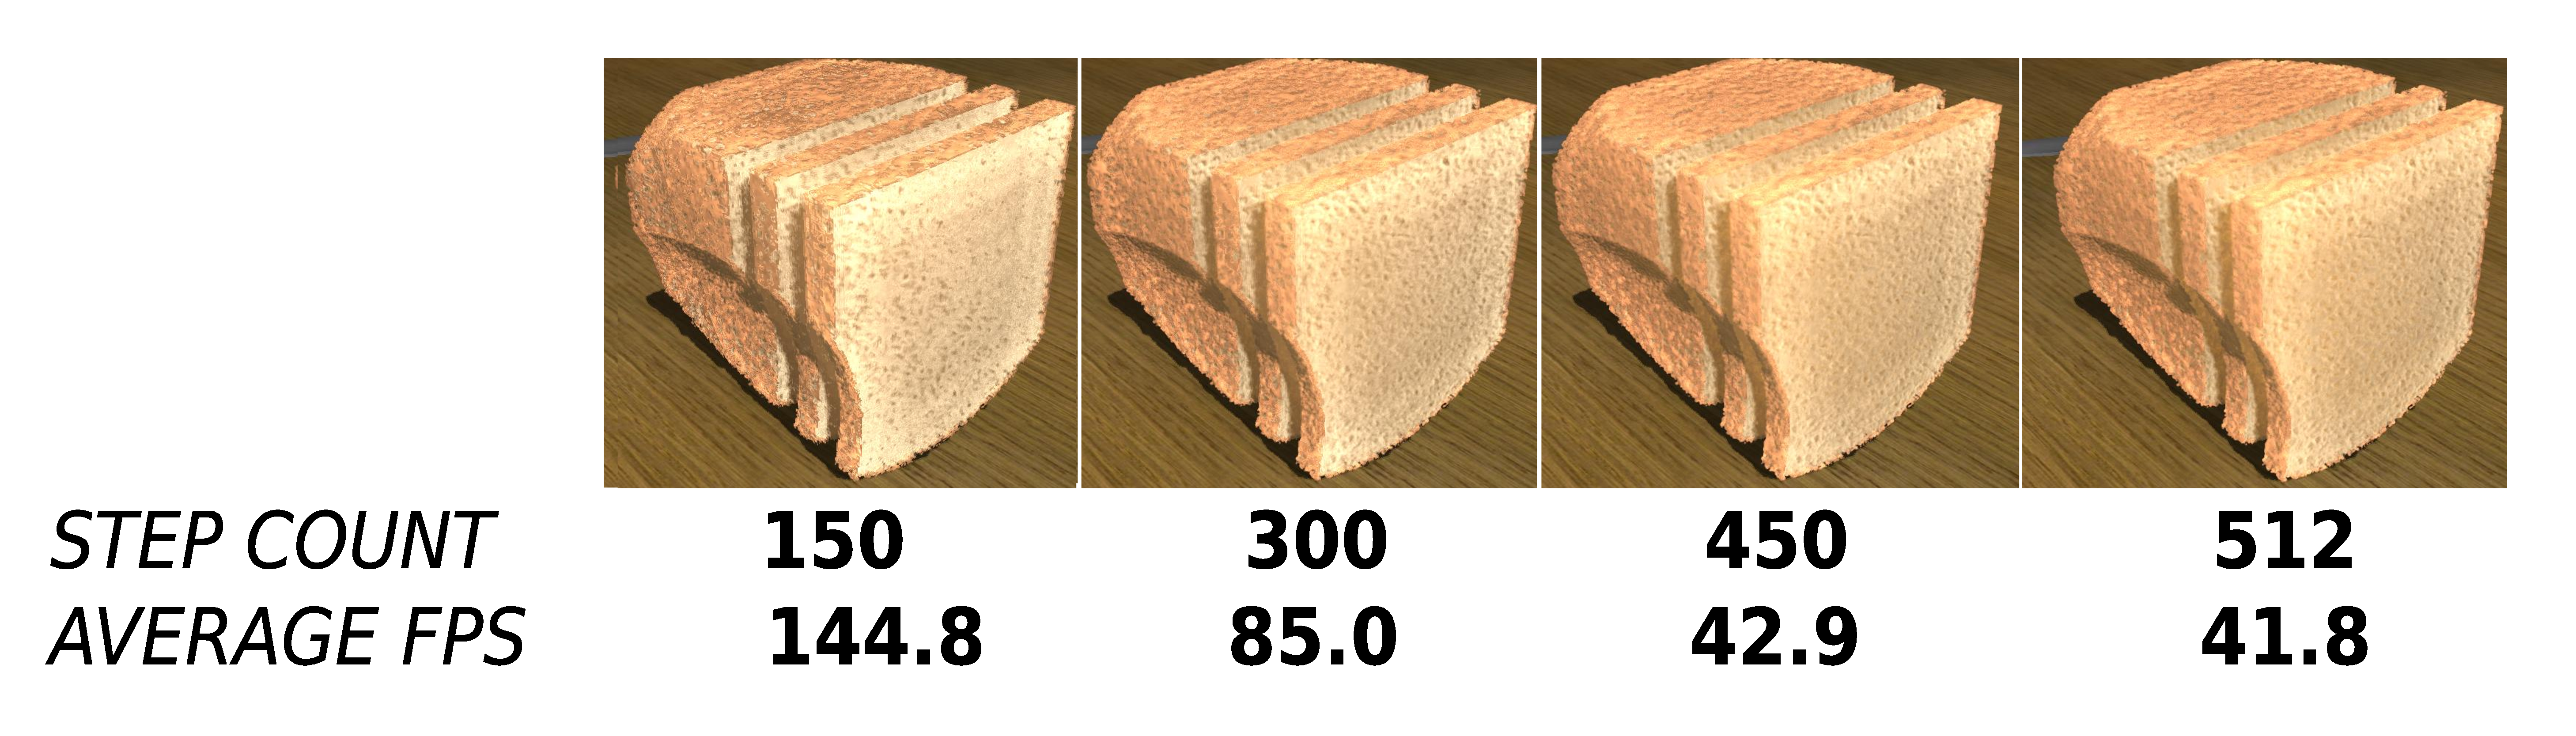
\includegraphics[width=13cm]{figures/stepcount}}
  \caption{Computing times and step count. The image shows that using $300$ sampling ray steps gives reasonably images. }
  \label{fg:stepcount}
\end{figure}

\begin{figure}
  \centerline{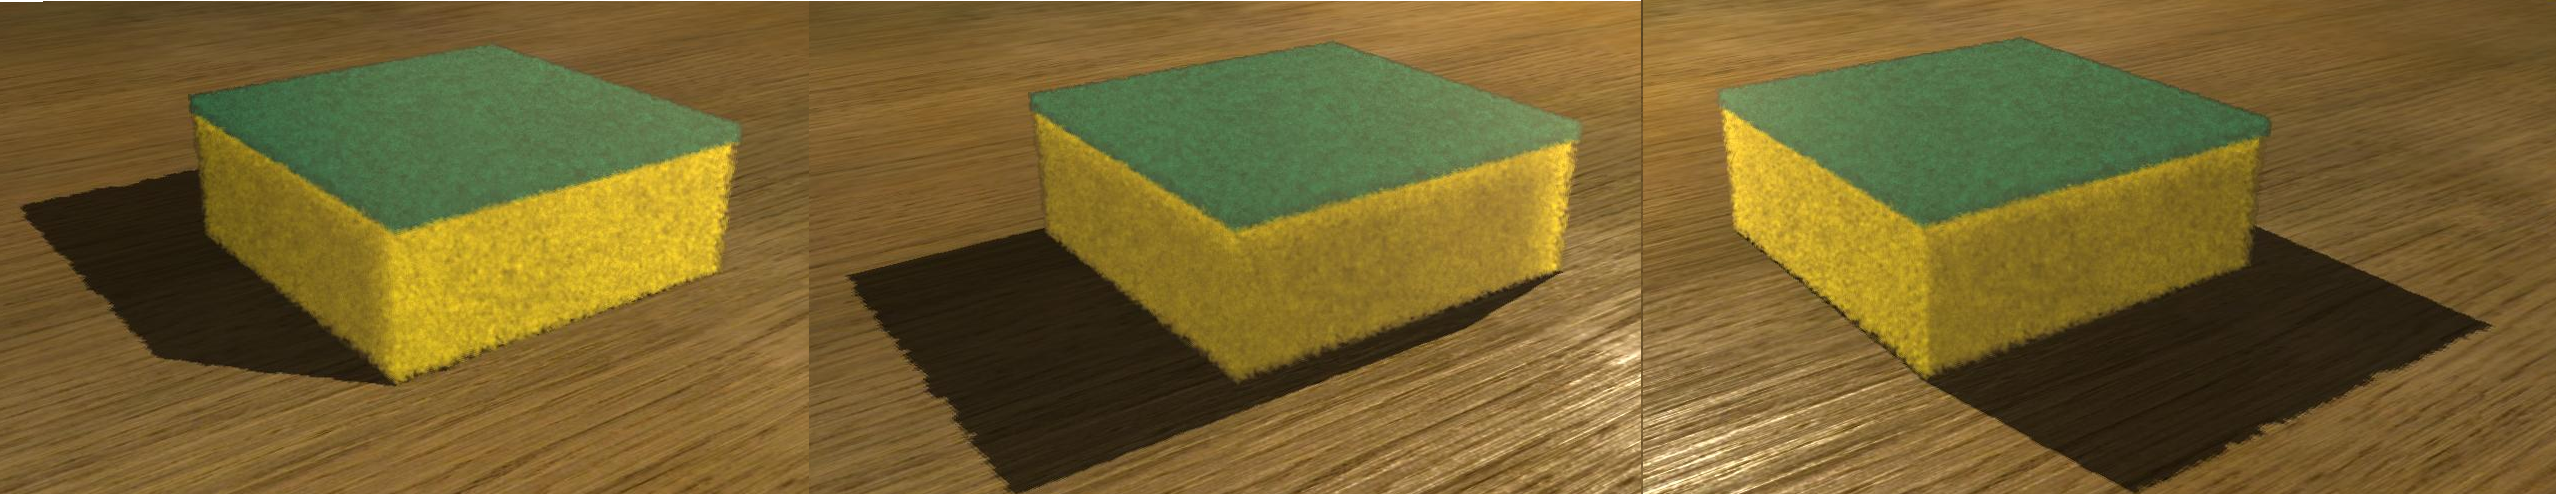
\includegraphics[width=13cm]{figures/sponges}}
  \caption{Real time rendered sponges using a random scalar field as geometry.}
  \label{fg:sponges}
\end{figure}


\begin{figure}
\centerline{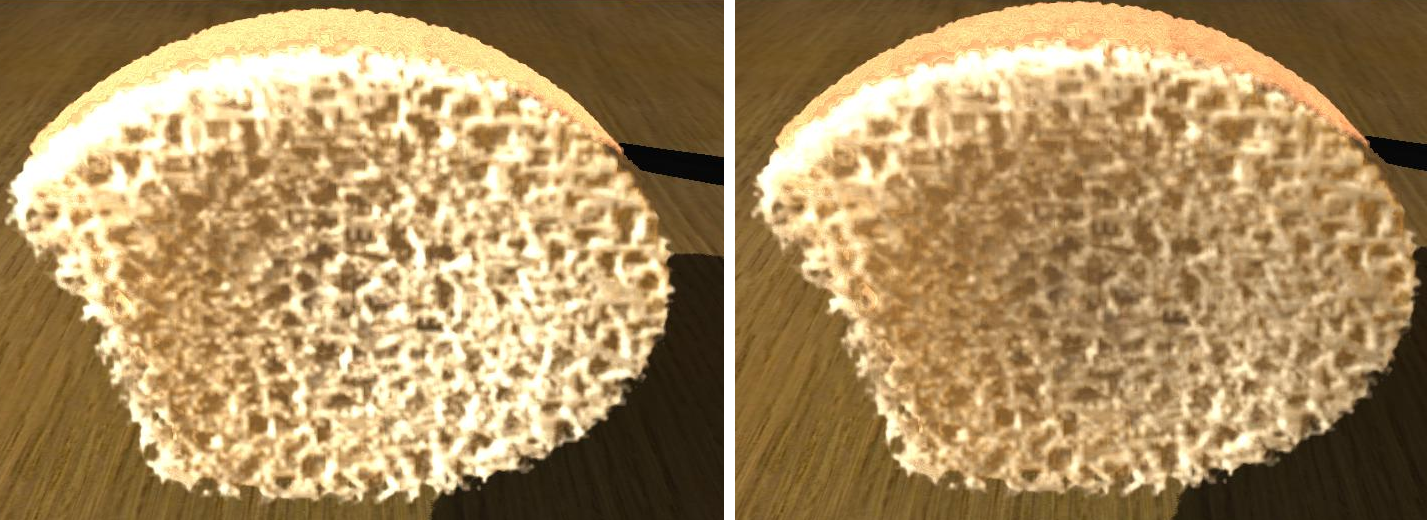
\includegraphics[width=13cm]{figures/occlusion}}
  \caption{Bread without (left) and with (right) ambient occlusion. The final appearance is greatly improved, showing a more natural look. }
  \label{fg:occlusion}
\end{figure}
